\documentclass[border=4pt,crop=true]{standalone}
\usepackage{pgfplots}
\pgfplotsset{compat=1.18}

% $|H|=\omega/\omega_0$, $G_{\mathrm{dB}}=20\log_{10}(\omega/\omega_0)$

\begin{document}
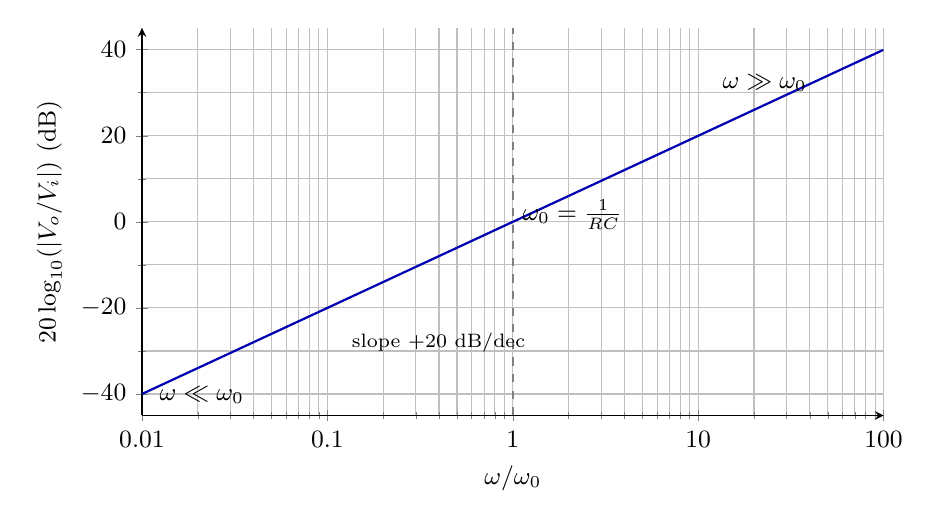
\begin{tikzpicture}
  \begin{axis}[
    width=11cm,
    height=6.5cm,
    xmode=log,
    xmin=1e-2,
    xmax=1e2,
    ymin=-45,
    ymax=45,
    axis lines=left,
    xlabel={$\omega/\omega_0$},
    ylabel={$20\log_{10}(|V_o/V_i|)$ (dB)},
    xtick={1e-2,1e-1,1,1e1,1e2},
    xticklabels={$0.01$,$0.1$,$1$,$10$,$100$},
    ytick={-40,-20,0,20,40},
    grid=both,
    minor tick num=1,
    tick label style={font=\small},
    label style={font=\small},
    every axis plot/.append style={thick},
  ]
    \addplot[blue!70!black,domain=1e-2:1e2,samples=300]
      {20*ln(x)/ln(10)};
    \addplot[gray,dashed] coordinates {(1,-45) (1,45)};
    \node[anchor=south west,font=\small] at (axis cs:1,-4)
      {$\omega_0=\frac{1}{RC}$};
    \node[anchor=north east,font=\small] at (axis cs:0.04,-36)
      {$\omega\ll\omega_0$};
    \node[anchor=south west,font=\small] at (axis cs:12,28)
      {$\omega\gg\omega_0$};
    \node[anchor=west,font=\scriptsize] at (axis cs:0.12,-28)
      {slope $+20$ dB/dec};
  \end{axis}
\end{tikzpicture}
\end{document}
